\documentclass[10pt]{article}
\usepackage[polish]{babel}
\usepackage[utf8]{inputenc}
\usepackage[T1]{fontenc}
\usepackage{amsmath}
\usepackage{amsfonts}
\usepackage{amssymb}
\usepackage[version=4]{mhchem}
\usepackage{stmaryrd}
\usepackage{graphicx}
\usepackage[export]{adjustbox}
\graphicspath{ {./images/} }

\begin{document}
\begin{enumerate}
  \item Znajdź wszystkie pary liczb całkowitych \((x, y)\), które spełniają równanie
\end{enumerate}

\[
12 x+18 y=20182018
\]

\begin{enumerate}
  \setcounter{enumi}{1}
  \item Rozstrzygnij, czy szachownicę \(8 \times 8\) z której usunięto pola A1 i H8 można pokryć kostkami domina, z których każde pokrywa dwa pola szachownicy i kostki na siebie nie zachodzą.
  \item W trójkącie \(A B C\) punkt \(H\) jest punktem przecięcia wysokości, a punkt O jest środkiem okręgu opisanego. Udowodnij, że kąty ACH i OCB są równe.\\
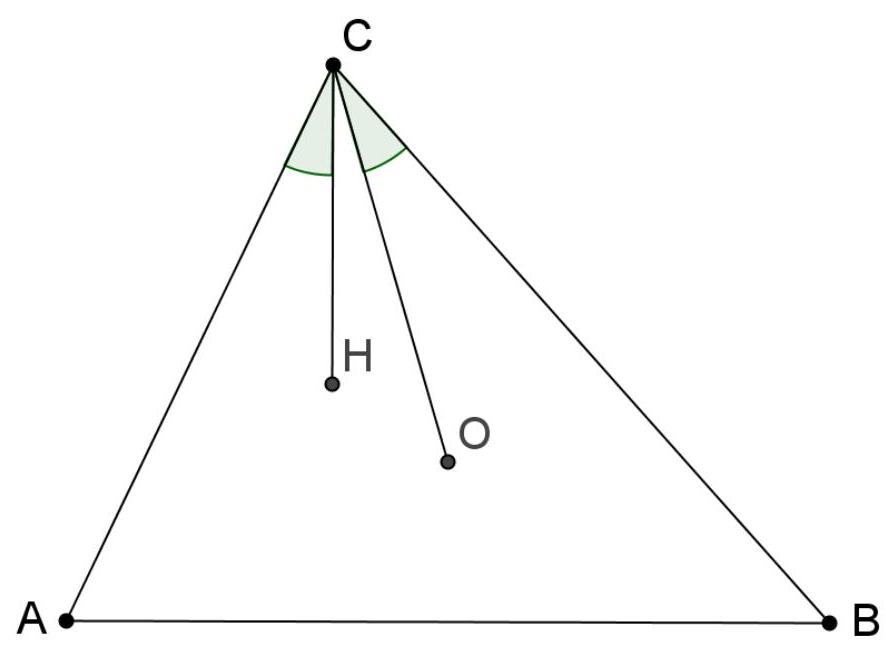
\includegraphics[max width=\textwidth, center]{2024_11_21_63b7cdbe3ba76a88bb7eg-1}
\end{enumerate}

\end{document}